\section{Organization and Management}
\label{sec:fdsp-tpcelec-management}

In this section we first discuss the organization of the \dword{tpc} electronics
consortium that at the moment consists entirely of US institutions: 
fifteen university groups plus groups from four DOE national 
laboratories. Table~\ref{tab:SPCE:institutions} provides a list 
of the participating institutions.
Later we discuss the assumptions that have been made in developing
the construction plan for the detector components that will be
provided by the \dword{tpc} electronics consortium, including the responsibilities
of the different institutions that are part of the consortium. Finally,
we present a schedule for the construction, integration, and installation
of the \dword{tpc} electronics into the detector. 

\begin{dunetable}
[Participating intitutions ]
{ll}
{tab:SPCE:institutions}
{Institutions participating in the \dword{tpc} electronics consortium (all from the US).}
Institution  \\ \toprowrule
Boston University \\ \colhline
Brookhaven National Laboratory \\ \colhline
%% University of Chicago \\ \colhline
University of Cincinnati \\ \colhline
Colorado State University  \\ \colhline
%% Columbia University \\ \colhline
University of California, Davis \\ \colhline
\dword{fnal} \\ \colhline
University of Florida \\ \colhline
University of Hawaii \\ \colhline
Iowa State University \\ \colhline
University of California, Irvine \\ \colhline
Lawrence Berkeley National Laboratory \\ \colhline
Louisiana State University \\ \colhline
Michigan State University \\ \colhline
University of Pennsylvania \\ \colhline
University of Pittsburgh \\ \colhline
SLAC National Accelerator Laboratory \\ \colhline
Stony Brook University \\
\end{dunetable}

%%%%%%%%%%%%%%%%%%%%%%%%%%%%%%%%%%%
\subsection{Consortium Organization}
\label{sec:fdsp-tpcelec-management-consort}

The present consortium organization
structure includes a consortium leader and a technical lead (both currently
from \dword{fnal}), with personnel from \dword{bnl} helping with system design. A working group structure has been recently 
provided with subgroups responsible for the detector 
components inside the cryostat (\dwords{asic}, \dwords{femb}, and
cold cables), outside the cryostat (mostly the \dwords{wiec} with 
their boards), and all equipment
used for testing the detector components. When appropriate, a subgroup
responsible for integration and installation activities at
\dword{surf} will be formed (for now, the technical lead oversees 
these activities). In addition,
another subgroup will be in charge of software and physics
preparation activities, including calibrations and simulations.
Mechanical design activities span detector components both inside
and outside the cryostat, requiring strong contacts between 
\dword{tc} and other consortia (mainly the \dword{apa}
consortium). The lead engineer (from \dword{bnl}) on mechanical aspects of the cold
electronics (mechanical interfaces with the \dword{apa}s, cabling, including 
cable trays, and cryostat penetrations) works directly with
the \dword{tc} team. The \dword{tpc} electronics consortium will also have 
contact people for the overall \dword{lbnf}/\dword{dune} management for
\dword{esh} and for \dword{qa}/\dword{qc}. For the moment, the technical lead oversees these activities, although oversight
will be transferred in part to each subgroup leader for testing
activities. The leadership positions in the consortium 
are listed in Table~\ref{tab:SPCE:leadership} and a diagram of
the organization of the consortium and of its relationships
with other groups in the \dword{lbnf} and \dword{dune} organizations
is shown in Figure~\ref{fig:sp-tpcelec-orgchart}.

\begin{dunetable}
[Leadership positions in the TPC electronics consortium]
{p{0.35\textwidth}}
{tab:SPCE:leadership}
{Current leadership positions in the TPC electronics consortium.}\
Position \\ \toprowrule
Consortium Leader \\ \colhline 
Technical Lead \\ \colhline 
System Aspects \\ \colhline 
Cold Components \\ \colhline 
Warm Components \\ \colhline 
Test Setups \\ \colhline 
Integration and Installation \\ \colhline
Mechanical Design \\ \colhline 
Reliability Task Force \\ \colhline 
TDR Editor \\ \colhline 
\dword{esh} contact \\ \colhline 
\dword{qa}/\dword{qc} contact \\
\end{dunetable}

\begin{dunefigure}
[Organization chart of the TPC electronics consortium]
{fig:sp-tpcelec-orgchart}
{Organization chart of the TPC electronics consortium and relations to
other groups in the \dword{lbnf} and \dword{dune} organizations (shown in green).}
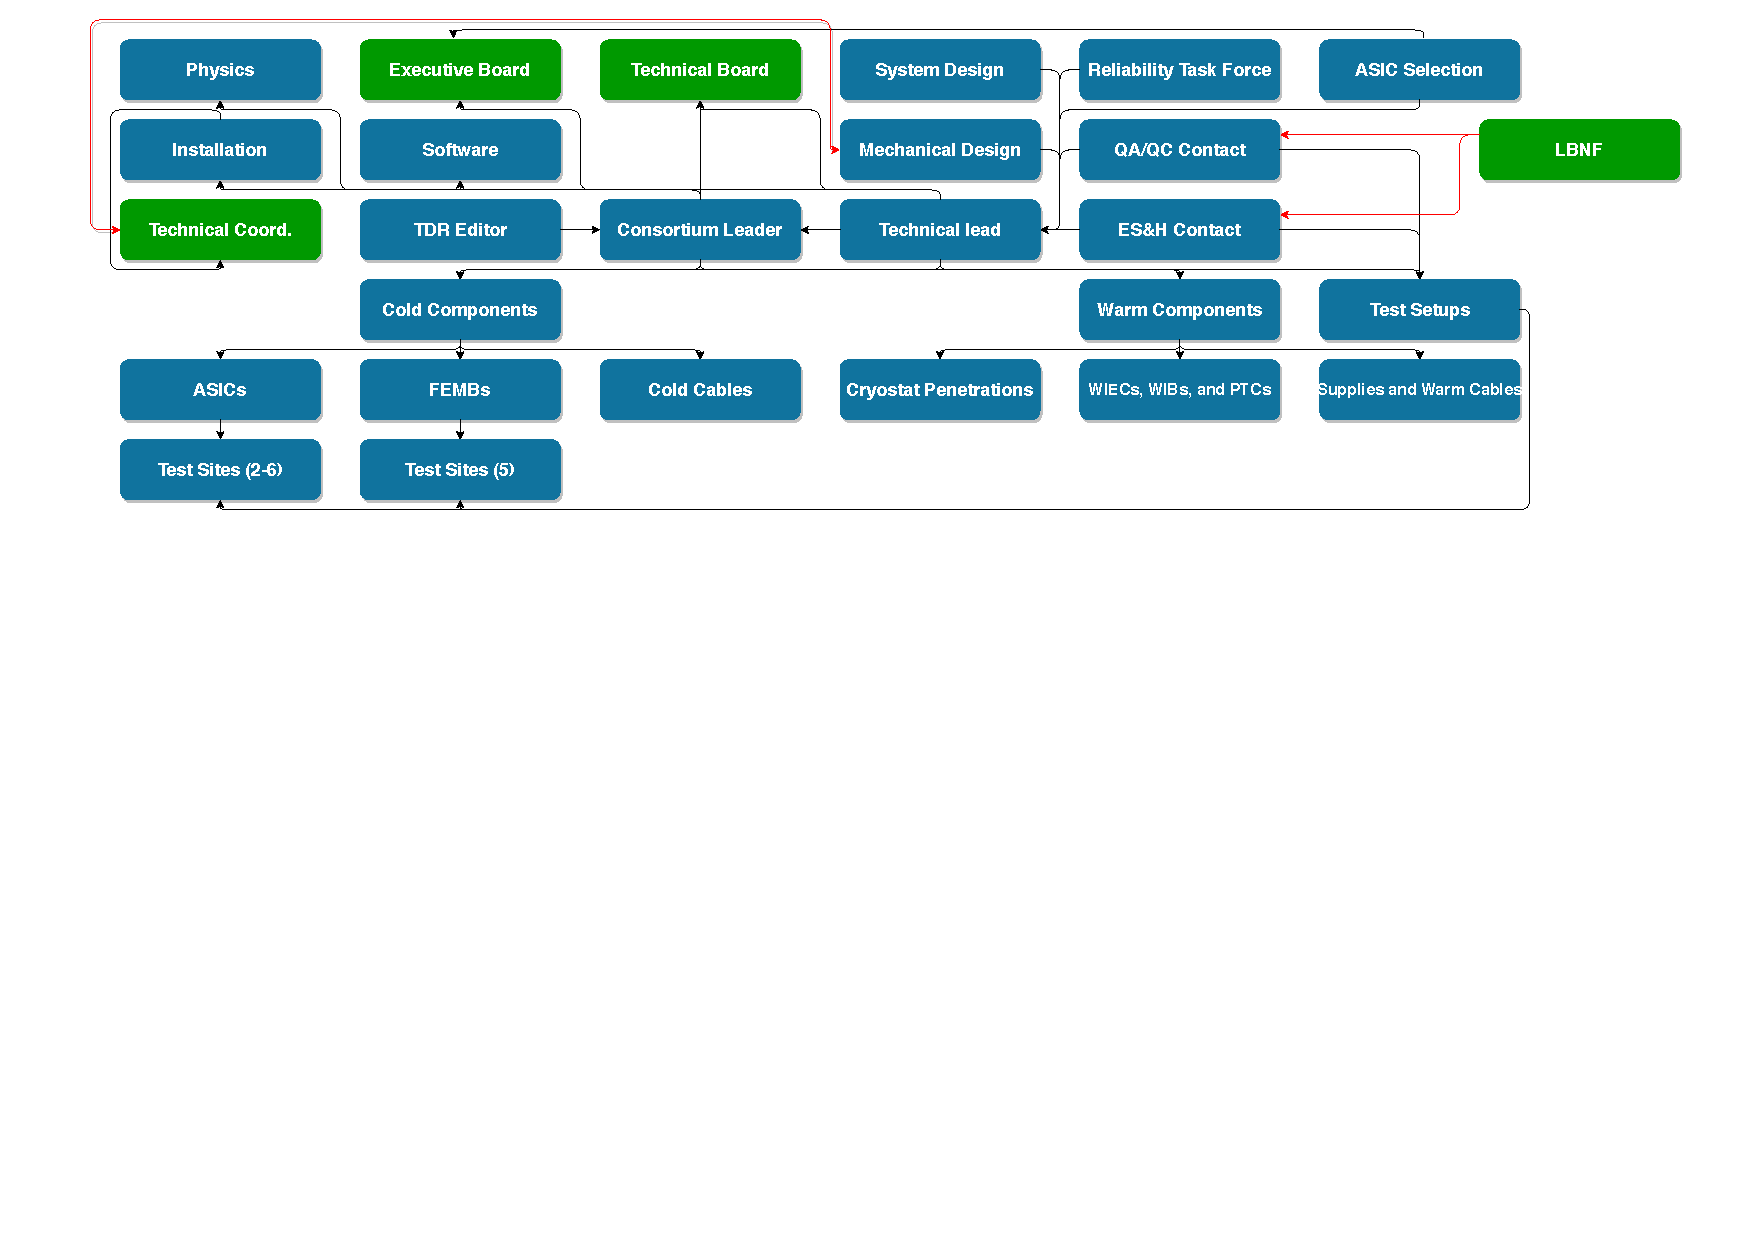
\includegraphics[width=\linewidth]{sp-tpcelec-orgchart.pdf}
\end{dunefigure}


In addition to the working groups, task forces for specific issues 
will be formed as necessary. A first example is the task force
charged with studying reliability issues in the \dword{tpc} electronics 
components and preparing recommendations for the choice of 
\dwords{asic}, the design of printed circuit boards, and testing; this
was discussed in Section~\ref{sec:fdsp-tpcelec-qa-reliability}. 
Later on, this task force will help in developing the \dword{qc} 
program for the \dword{tpc} electronics detector components in collaboration
with the testing group leadership, with the \dword{pdsp} 
experience as a starting point. Later, a second task force, with possible
personnel overlap with the first task force and possibly including experts
from outside of the \dword{dune} Collaboration, will be tasked with establishing the
criteria for the \dword{asic} selection. This task force will
be also asked to propose a recommendation that will then go to
the \dword{dune} Executive Board for the final approval, as discussed
in Section~\ref{sec:fdsp-tpcelec-design-femb-selection}.

%%%%%%%%%%%%%%%%%%%%%%%%%%%%%%%%%%%
\subsection{Planning Assumptions}
\label{sec:fdsp-tpcelec-management-planning}

In Section~\ref{sec:fdsp-tpcelec-management-cost}, we describe
the current schedule for the construction, integration, and installation
of the \dword{tpc} electronics detector components for the first \dword{sp} \dword{tpc}
\dword{fd} module. This schedule, as well as the costs associated
with detector construction, are based on experience with constructing
and commissioning the \dword{pdsp}
detector in addition to assumptions for the remaining R\&D program
and the production planning discussed here. 
Section~\ref{sec:fdsp-tpcelec-production-spares} details
the number of spare parts that we plan to fabricate in order to
account for known yield issues during detector construction
and to address possible problems. Table~\ref{tab:SPCE:components}
gives a summary of all fabricated components required for the first \dword{sp}
\dword{fd} module. To develop a schedule for detector construction, 
we must consider the current state of development of 
the \dwords{asic}, \dwords{femb}, and all other components in order to 
estimate the time required for the final production.

A second detector module may be built using the \dword{sp} technology, 
and in that case the construction of the \dword{tpc} electronics components 
for the second module would immediately follow construction of 
the first one. The total number of components for the second 
module will be less than the amount for the first detector, assuming that 
for components inside the cryostat the spare parts from the first 
module can be used for the second. Similarly, for the 
components on the top of the cryostat, the pool of spares from the 
first module should be sufficient to cover the second.
Given the timeline for the construction of the detector components
and their integration on the \dword{apa}s or their installation at
\dword{surf}, an insufficient number of spares presents a risk only
for the second detector module, as discussed in Section~\ref{sec:fdsp-tpcelec-risks-design}.

The critical path for the construction of the first \dword{sp}
\dword{tpc} \dword{fd} module is driven by the availability of \dwords{femb},
which in turn depends on completing the design of the
\dwords{asic}. Thus, construction
of the \dword{apa}s could start as early as spring 2020, while the
decision on the \dwords{asic} to be used on the \dwords{femb}
may come as late as January 2021. The schedule for this decision
depends on the \dword{tpc} electronics consortium, which is
planning a second design iteration on all \dwords{asic}
followed by system tests of various flavors of \dwords{femb}.
The first version of all \dwords{asic} has been undergoing
standalone tests in spring / summer 2019 and then will go through the 
sequence of system tests (with the 40\% \dword{apa} prototype at \dword{bnl},
the seventh \dword{pdsp} \dword{apa} in the cold box at CERN,
and the \dword{tpc} in the \dword{iceberg} cryostat at \dword{fnal})
during fall / winter 2019. At the same time, lifetime tests will be performed 
on all \dwords{asic}. Designs of the \dwords{asic} and \dwords{femb}, including results
from the system test stands and from lifetime tests, will be reviewed
in early 2020. This will trigger any further design
changes on the \dwords{asic}, to be followed by a second round of prototyping
and testing. This gets us to the January 2021 date for the final
\dword{asic} decision. Consequently, the initial
tests of the \dword{dune} prototype \dword{apa}s must be performed
with preliminary versions of \dwords{femb}, which will still be using
the first generation of \dwords{asic} (although the final 
mechanical and electrical connections to the \dword{apa}s will be available and used).

\begin{dunetable}[Number of TPC electronics components for one detector module]
{p{0.5\textwidth}p{0.5\textwidth}}
{tab:SPCE:components}
{Number of TPC electronics components required for a full \dword{spmod} (accounting for spares and yields during \dword{qc}).}
Detector component & Number required \\ \toprowrule
\dword{larasic} & 30,000 chips (at least 43 wafers) \\ \colhline
\dword{coldadc} and \dword{coldata} & 30,000 and 7,500 chips (at least 33 wafers) \\ \colhline
\dword{cryo} & 7,500 chips (at least 35 wafers) \\ \colhline
\dword{femb} & 3,200 \\ \colhline
Cold signal cables & 1,650 and 1,575 (bottom and top \dword{apa}) \\ \colhline
Cold power cables & 1,650 and 1,575 (bottom and top \dword{apa}) \\ \colhline
Cold bias voltage cables & 660 and 630 (bottom and top \dword{apa}) \\ \colhline
Cryostat penetrations & 80 \\ \colhline
\dword{ce} flanges & 160 \\ \colhline
\dword{wiec} & 155 \\ \colhline
\dword{wib} & 775 \\ \colhline
\dword{ptc} & 155 \\ \colhline
Warm power cables & 165 (three different lengths) \\ \colhline
Warm bias voltage cables & 1,320 (three different lengths) \\ \colhline
Wiener PL506 power box & 30 \\ \colhline
Wiener MPOD crate & 30 \\ \colhline
Wiener MPOD modules with 8 HV channels & 180 \\ \colhline
Power supplies and cables for heaters and fans & 30 \\
\end{dunetable}

After the January 2021 review, an additional six months may be 
required for a final iteration of the \dword{femb} design
and a final round of system tests before beginning fabrication
of the \dwords{asic} and \dwords{femb}. Engineering runs
for the \dwords{asic} and \dwords{femb} should then take place in the
second half of 2021, with most production starting in
spring 2022. Production and testing of all chips required
for constructing the first \dword{sp} \dword{tpc} \dword{fd} module
would be completed by August 2023. The first batch of
production \dwords{femb} would then be available for installation on
the \dword{apa}s in February 2023, and production would be
completed in January 2024, roughly eight months before the 
beginning of the integration of the \dwords{femb} on the
\dword{apa}s at \dword{surf}. The final \dwords{femb} for the 
first \dword{spmod} are expected to be available at the \dword{sdwf} 
fourteen months ahead of their for installation on the 
last \dword{apa} to be installed inside the cryostat.
There are therefore between eight and fourteen months of float
in the schedule for the \dwords{asic} and \dwords{femb}, which 
would allow for a third iteration of design and prototyping
if needed. It should be noted that, for the detector components
to be installed on the top of the cryostat, there are between
ten and fourteen months of float.

The schedule presented above assumes that during the
construction of the \dword{apa}s,
integration tests will be performed using preliminary
versions of the \dwords{femb} that must then be replaced
with final versions at a later date. It also assumes that for the
second run of \dword{pdsp}, expected to take place in the
second half of 2021, prototype \dwords{femb} using the
second iteration of prototype \dwords{asic} will be used.
Using the \dwords{asic} from the pre-production, fabricated using
the masks that will be used during the production phase, 
would require a delay of one year in the second run of
\dword{pdsp}. The difference in the masks used for the
fabrication of the \dwords{asic} (multipurpose wafer run instead 
of a dedicated run) does not negate the usefulness of
the second run of \dword{pdsp} as a final validation of
the \dword{dune} \dword{spmod} design.

If a second \dword{sp} \dword{tpc} \dword{fd} module is built, the critical
path will transition from the \dwords{femb}
to the \dword{apa}s, assuming that construction
of both \dword{apa}s and \dwords{femb} will continue 
without interruption after construction of the first module. 
This is because constructing one \dword{apa} requires 
more time than constructing the corresponding \dwords{femb}. Therefore,
toward the end of the constructing this possible second module,
we expect that all required \dwords{femb} will be at the
\dword{sdwf} waiting for the delivery of the \dword{apa}s before
integration can take place.

All other detector components that are the responsibility of the
\dword{tpc} electronics consortium can be produced relatively quickly
in less than two years. The procurement, assembly, and
testing of these components can be scheduled so that
we have sufficient time in the schedule to address possible 
problems during production. Changes in all of these
components, unlike those used in the \dword{pdsp} detector,
are less important than those affecting the \dwords{asic}
and \dwords{femb}. We are assuming that final
designs for the rest of the detector components will be 
available in the second half of 2020 and that the corresponding 
production readiness reviews will occur, at the latest, six months 
before the \dword{asic} design choice.
The first components to be installed on the detector are the cryostat
penetrations, which must be installed before the 
detector support structure inside the cryostat is completed.
In this way, the cryostat can be completely sealed, other than
the manholes used to feed clean air into the cryostat
and the \dword{tco} that is used as an exhaust portal 
and as an entry point for the detector components. The rest of the
\dword{tpc} electronics components, which are installed on top of the 
cryostat (\dwords{wiec} with all of their boards, supplies, cables,
and fibers), should be installed before installing
the corresponding rows of \dword{apa}s and properly connecting
the cables linking the \dword{apa}s to power, control, and readout. 
The \dword{apa}s should be tested as soon as they are installed. 

%%%%%%%%%%%%%%%%%%%%%%%%%%%%%%%%%%%
\subsection{Institutional Responsibilities}
\label{sec:fdsp-tpcelec-management-resp}

Design and prototyping for the \dword{sp} \dword{dune} \dword{fd} have been 
concentrated so far at the DOE national laboratories, mostly because the 
focus has been on designing the new generation of \dwords{asic}. The design 
of the \dword{larasic} was done at \dword{bnl}, the \dword{cryo} 
chip was done at \dword{slac}, and the new \dword{coldadc} was a joint effort of 
\dword{bnl}, \dword{fnal}, and \dword{lbnl}. The \dword{coldata} 
\dword{asic} was designed at \dword{fnal}, with some components 
provided by engineers from the Electrical Engineering Department
at Southern Methodist University (not a consortium member).
The \dword{cts} was designed at Michigan State University.
Most of the design and construction work for the \dword{pdsp} detector 
was done at \dword{bnl}, with other institutions contributing to 
testing, installation, and commissioning. Given the extent of the project, 
particularly testing, additional institutions have begun to contribute
to all of the activities for constructing the \dword{dune} \dword{sp} \dword{fd}, which began 
in the middle of 2018. Almost all the engineering of detector components, 
except for the boards to be installed on the \dwords{wiec} and most boards 
and setups for testing, will remain a responsibility
of the DOE national laboratories. Testing of 
\dwords{asic}, \dwords{femb}, cables, power and bias voltage supplies,
and \dwords{wiec} with their boards will be done at various
universities that are members of the consortium. All institutions
are expected to contribute to the integration and installation activities at
at \dword{surf}, which is very
demanding in terms of personnel. A detailed list of the 
institutions contributing to the development, production, and
testing of the various detector components is given in Figure~\ref{fig:sp-tpcelec-responsibilities}.

\begin{dunefigure}
[Construction responsibilities for the TPC electronics consortium]
{fig:sp-tpcelec-responsibilities}
{Responsibilities of the institutions in the \dword{tpc} electronics 
consortium, matched to the organization chart of the consortium.}
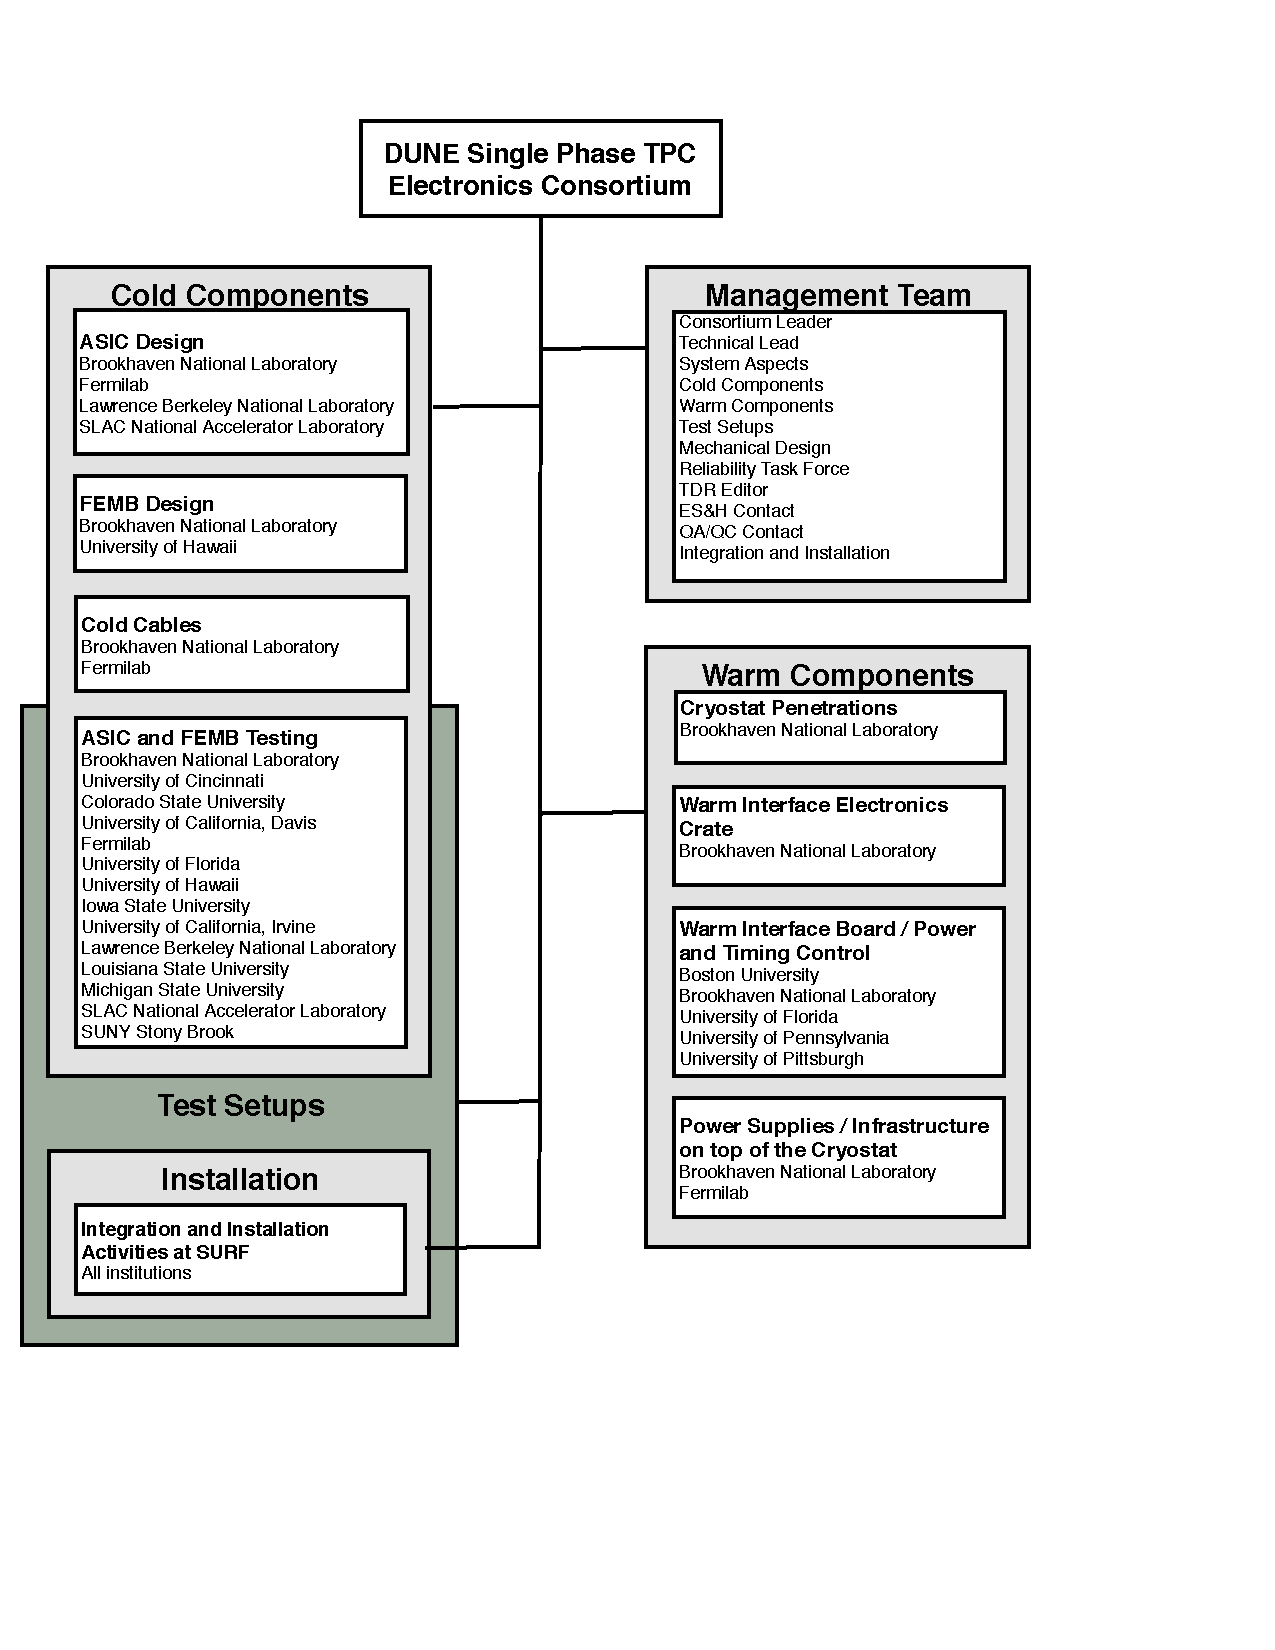
\includegraphics[width=0.8\linewidth]{sp-tpcelec-responsibilities.pdf}
\end{dunefigure}

%%%%%%%%%%%%%%%%%%%%%%%%%%%%%%%%%%%
\subsection{High-Level Cost and Schedule}
\label{sec:fdsp-tpcelec-management-cost}

\begin{dunetable}
[TPC electronics consortium milestones]
{p{0.75\textwidth}p{0.20\textwidth}}
{tab:SPCE:timeline}
{Milestones of the TPC electronics consortium.}
Milestone & Date \\ \toprowrule
Complete the submission of the first generation of \dwords{asic} & April 2019\\ \colhline
Complete the standalone testing of the first generation of \dwords{asic} & October 2019\\ \colhline
Complete system and lifetime tests on the first generation of \dwords{asic} and \dwords{femb} & January 2020\\ \colhline
Submission of second generation of \dwords{asic} & March 2020 \\ \colhline
Complete the standalone testing of the second generation of \dwords{asic} & September 2020 \\ \colhline
Complete system and lifetime tests on the second generation of \dwords{asic} and \dwords{femb} & January 2021\\ \colhline
Decision on the \dword{asic}(s) to be used for construction &  January 2021\\ \colhline
\rowcolor{dunepeach} Start of \dword{pdsp}-II installation& \startpduneiispinstall      \\ \colhline
Complete characterization of final prototypes of \dwords{asic} and \dwords{femb} including system tests & July 2021\\  \colhline
Complete Engineering Design Reviews and launch pre-production of detector components & September 2021 \\ \colhline
Start of procurement of cold cables & December 2021 \\ \colhline
Start of production of cryostat penetrations & December 2021 \\ \colhline
Start of production of \dwords{wiec}, \dwords{wib}, and \dwords{ptc} & December 2021 \\ \colhline
Start of procurement of power supplies and warm cables & December 2021 \\ \colhline
Complete testing of pre-production of all \dwords{asic} & January 2022\\ \colhline
Complete testing of pre-production \dwords{femb} & April 2022 \\ \colhline
\rowcolor{dunepeach}South Dakota Logistics Warehouse available& \sdlwavailable      \\ \colhline
Complete testing of prototypes and Production Readiness Reviews & May 2022\\ \colhline
Start of \dwords{asic} production & May 2022 \\ \colhline
Start of \dwords{femb} production & May 2022 \\ \colhline
\rowcolor{dunepeach}Beneficial occupancy of cavern 1 and \dword{cuc}& \cucbenocc      \\ \colhline
Completion of cryostat penetrations procurement & February 2023 \\ \colhline
Completion of the procurement and \dword{qc} of cold cables & March 2023 \\ \colhline
\rowcolor{dunepeach} \dword{cuc} counting room accessible& \accesscuccountrm      \\ \colhline
Completion of the \dwords{wiec}, \dwords{wib}, and \dwords{ptc} production and \dword{qc} & May 2023 \\ \colhline
Completion of the procurement of power supplies and warm cables & June 2023 \\ \colhline
Completion of \dwords{asic} production and \dword{qc} & August 2023 \\ \colhline
Completion of \dwords{femb} production and \dword{qc} & January 2024 \\ \colhline
Begin installation of the \dword{tpc} electronics components on top of the cryostat & April 2024 \\ \colhline
Complete installation of the \dword{tpc} electronics components on top of the cryostat & July 2024 \\ \colhline
\rowcolor{dunepeach}Start of \dword{detmodule} \#1 TPC installation& \startfirsttpcinstall      \\ \colhline
Begin integration of the \dwords{femb} on the \dword{apa}s at \dword{surf} & August 2024 \\ \colhline
Complete integration of the \dwords{femb} on the \dword{apa}s at \dword{surf} &  March 2025\\ \colhline
\rowcolor{dunepeach}End of \dword{detmodule} \#1 TPC installation& \firsttpcinstallend \\
\end{dunetable}

In Section~\ref{sec:fdsp-tpcelec-management-planning}, we  
discussed how the project will evolve from the current design
and prototyping phase to production for the \dwords{asic}
and \dwords{femb} by spring 2022. During the same  
period, the engineering of all other detector components will
be completed and prototypes fabricated. The procurement
and qualification of cold cables, cryostat penetrations, \dwords{wiec},
and power and bias voltage supplies can then begin in spring 2021.
Integrating \dwords{femb} on the \dword{apa}s would then
take place over 18 months beginning in early 2023. At
this moment, the installation and testing of \dword{apa}s in 
the cryostat and corresponding activities of the \dword{tpc} electronics consortium, including installing all 
detector components on top of the cryostat, are scheduled to
take four months starting in April 2024. Table~\ref{tab:SPCE:timeline} shows a preliminary list of 
milestones, including the current plan to complete  
the design, R\&D, and engineering phases; and then later  
the production setup, production, integration,
and installation activities. The schedule for the 
completion of the design and prototyping, the pre-production,
the construction of the detector components (including the
\dword{qc} process), and their integration and installation at
\dword{surf} is displayed in Figure~\ref{fig:sp-tpcelec-schedule}.

\begin{dunefigure}
[Schedule for the construction of the TPC electronics detector components]
{fig:sp-tpcelec-schedule}
{Schedule for the completion of the design and prototyping, the pre-production,
the construction of the \dword{tpc} electronics detector components (including the
\dword{qc} process), and their integration and installation at \dword{surf}.}
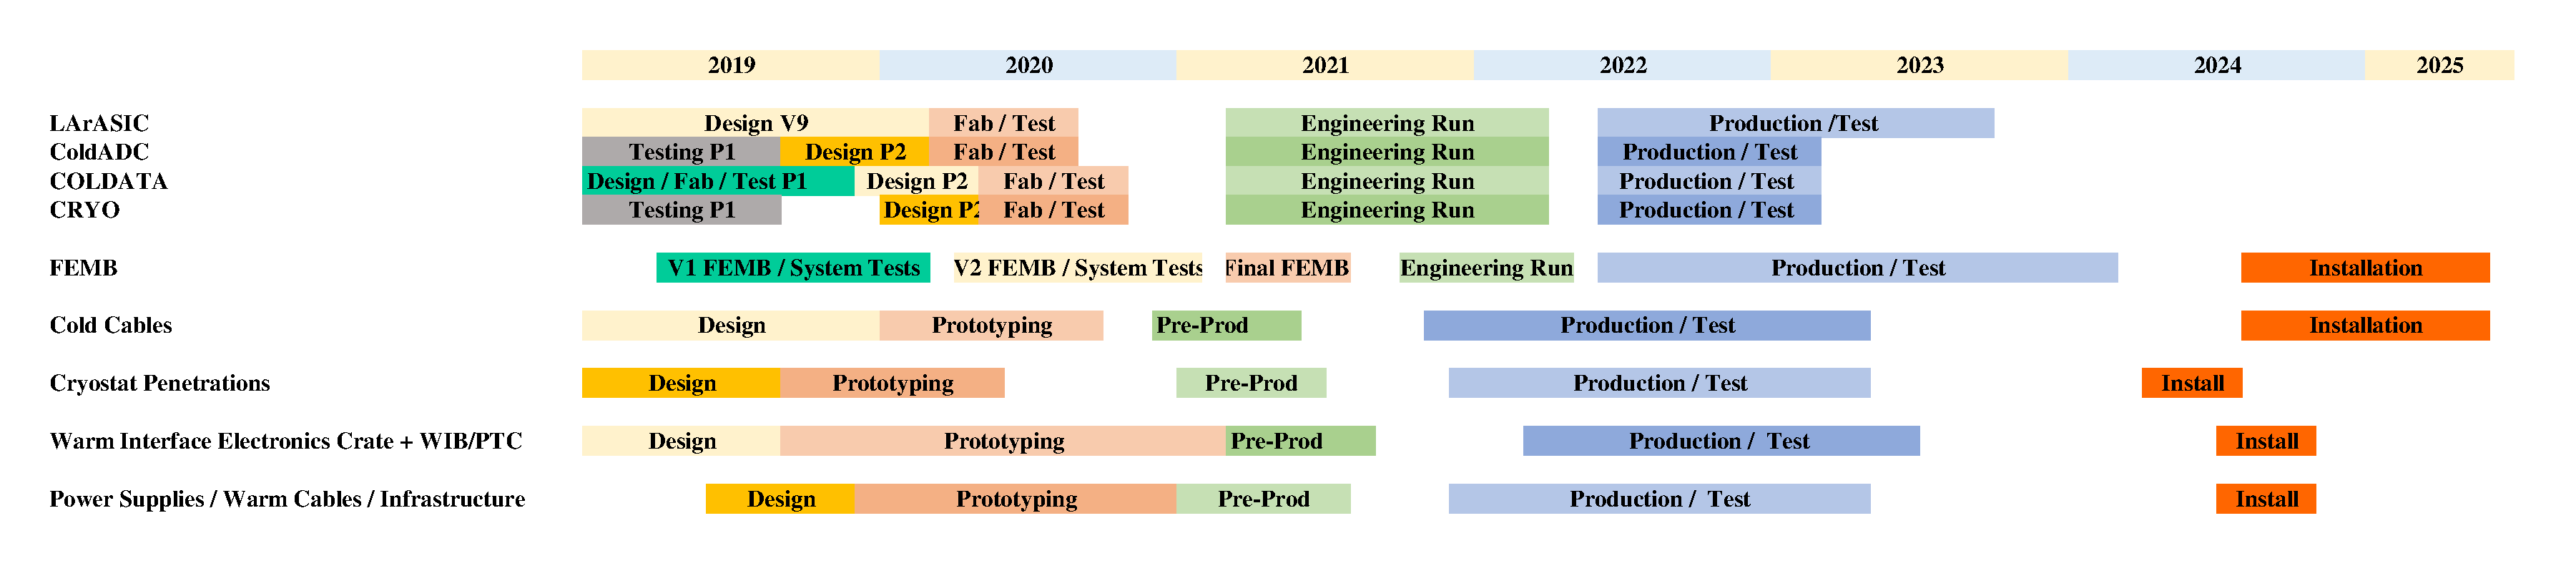
\includegraphics[width=\linewidth]{sp-tpcelec-schedule.pdf}
\end{dunefigure}

